\textbf{{1. 网桥的基本概念}}

{{\textbf{a.
基本介绍:}}在数据链路层扩展局域网是使用网桥。}{{\textbf{网桥}}\textbf{工作在数据链路层,其特点是具有过滤帧的功能}。网桥至少有两个端口,每个端口与一个网段相}{连。}

{\textbf{b.网桥的优点:}}{过滤通信量;}{扩大了物理范围;}{提高了可靠性;}{可互连不同物理层、不同MAC子层和不同速率(如10Mbit/s和100Mbit/s)的以太网。}

{\textbf{c.网桥的缺点:}}{存储转发增加了时延;}{在MAC子层并没有流量控制功能;}{具有不同MAC子层的网段桥接在一起时时延更大;}{网桥只适合于用户数不太多(不超过几百个)和通信量不太大的局域网,否则有时还会因传播过多的广播信息而产生网络拥塞,即广播风暴。}

\textbf{{2. 网桥的基本原理}}

{网桥每从一个端口接收到一个帧,就先暂存到缓存中。若该帧未出现差错,且欲发往的目的站MAC地址属于另一个网段(同一个网段无需转发,应该丢弃),则通过查找转发表,将该帧从对应的端口发出。因此,仅在同一个网段中通信的帧,不会被网桥转发到另一个网段中,因而不会加重整个网络的负担。}\textbf{网桥的内部结构}{如下图所示。}

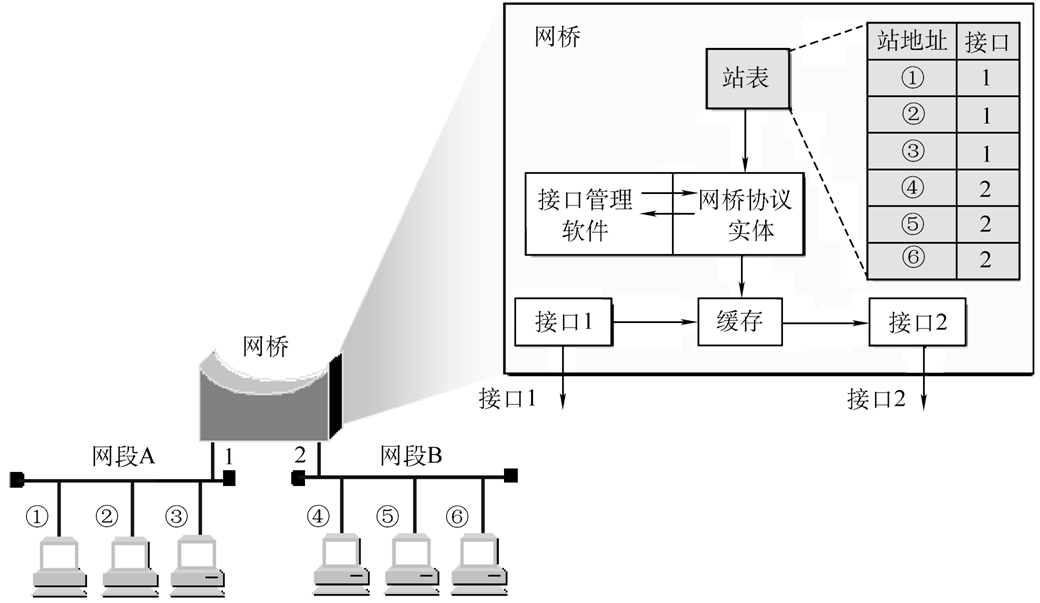
\includegraphics[width=3.33333in,height=1.93750in]{png-jpeg-pics/9E6C6903CF9DA9A3638270B546273ACD.png}
